\documentclass[10pt,a4paper]{article}
\usepackage[margin=2.2cm]{geometry}
\usepackage[utf8]{inputenc}
\usepackage[T1]{fontenc}
\usepackage{lmodern}
\usepackage{amsmath}
\usepackage{graphicx}
\usepackage{booktabs}
\usepackage{multirow}
\usepackage{xcolor}
\usepackage[hidelinks]{hyperref}
\usepackage[numbers,sort&compress]{natbib}
\usepackage{tikz}
\usetikzlibrary{arrows.meta,positioning}
\graphicspath{{figures/}}

\title{\textbf{SimADL-Health}: Simulating Long-Term Daily-Living Logs with Health Anomalies\\
to Detect, Attribute and Report Behaviour Change before a GP Consultation}
\author{SimADL-Health contributors\\ \small \url{https://github.com/ZeeetOne/SimADL-Health}}
\date{October 2026 --- technical report}

\begin{document}
\maketitle

\begin{abstract}
Health decline in older adults living alone is often noticed late: symptoms are under-reported or atypical, and a short
GP consultation does not show weeks of behaviour change. We build a compact, end-to-end prototype of the pipeline
targeted by the ObsAVQ project: from a list of daily-living events (sleep, eating, social interaction) to a report the GP
can read before the consultation. Because long-term labelled data are scarce, we (i)~calibrate a schedule-based simulator
on two real single-resident CASAS homes, (ii)~inject urinary tract infection (UTI), depression and mild cognitive decline
as parameter changes taken from a literature-tagged symptom catalogue, (iii)~detect changes against each person's own
baseline, (iv)~attribute them to a condition with a random forest explained by SHAP, and (v)~generate template-based
reports every 35~days. Simulated normal behaviour is as close to a held-out real year as two real years of the same person
are to each other (mean KS $D$ 0.188 vs 0.199). Attribution transfers across persons (macro-F1 0.58--0.59 when training on
one home and testing on the other; cognitive decline episodes always recognised). At a clinically tolerable rate of
false reports, however, report-level sensitivity remains modest, and on real residents a fixed baseline turns habit
drift into spurious ``cognitive decline''. We report these limits explicitly, as they define the open questions
for future work on ObsAVQ.
\end{abstract}

% ---------------------------------------------------------------------------------------------------------------
\section{Introduction}
Ambient monitoring of older adults at home can reveal changes in sleep, eating and social life that precede a clinical
problem. UTI is a typical example: in older adults it often presents atypically, yet it leaves traces in night-time
bathroom use~\cite{capstick2024uti,ugwu2026clinician}. Depression and cognitive decline reduce time out of home and
disturb routines~\cite{petersen2015timeout}. The ObsAVQ project aims at an automatic \emph{pre-consultation report} on
these activities of daily living (ADL), assuming that a recognition layer (e.g.\ audio) already provides a list of
timestamped events, and that long-term behaviour must be modelled on synthetic data because real labelled data are rare.

This report describes a one-week prototype of that idea, organised as the three objectives of the ObsAVQ project:
\textbf{O1} a generator of long-term ADL logs with health anomalies, \textbf{O2} ML methods that detect and attribute
changes and write the report, and \textbf{O3} an evaluation against prior work. Our contributions are:
(1)~a simulator calibrated on real older adults, with symptom parameters tagged by evidence level;
(2)~a per-person detection and attribution pipeline tested on an unseen person;
(3)~a periodic report (HTML and PDF) whose design follows deployed monitoring systems;
(4)~an honest evaluation, including a first sim-to-real check on two real residents.
Code, data processing and all figures are in the repository.

\begin{figure}[h]
\centering
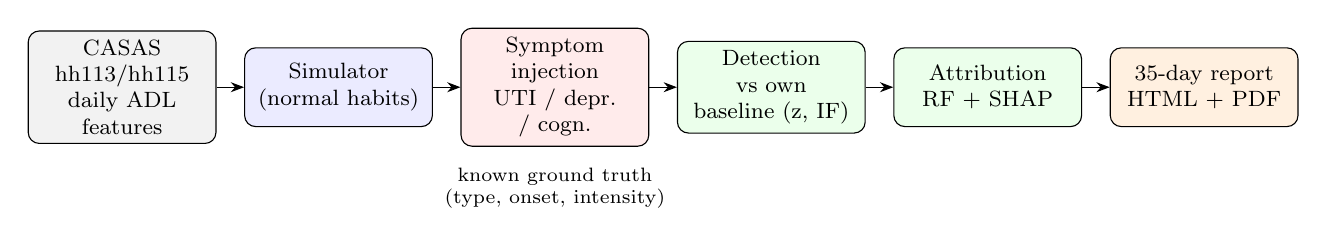
\begin{tikzpicture}[node distance=0.35cm, box/.style={draw, rounded corners, align=center, font=\footnotesize,
  minimum height=1.0cm, text width=2.15cm, fill=#1}, box/.default=white, >=Stealth]
\node[box=gray!10] (cal) {CASAS hh113/hh115\\daily ADL features};
\node[box=blue!8, right=of cal] (sim) {Simulator\\(normal habits)};
\node[box=red!8, right=of sim] (inj) {Symptom injection\\UTI / depr. / cogn.};
\node[box=green!8, right=of inj] (det) {Detection vs own\\baseline (z, IF)};
\node[box=green!8, right=of det] (att) {Attribution\\RF + SHAP};
\node[box=orange!12, right=of att] (rep) {35-day report\\HTML + PDF};
\draw[->] (cal) -- (sim); \draw[->] (sim) -- (inj); \draw[->] (inj) -- (det);
\draw[->] (det) -- (att); \draw[->] (att) -- (rep);
\node[font=\scriptsize, below=0.15cm of inj, text width=4cm, align=center] {known ground truth\\(type, onset, intensity)};
\end{tikzpicture}
\caption{Pipeline. Models are trained once on synthetic data and then applied to any person's event list.}
\label{fig:pipeline}
\end{figure}

% ---------------------------------------------------------------------------------------------------------------
\section{Related work}
\textbf{Synthetic smart-home data.} SynSys~\cite{dahmen2019synsys} trains HMMs and regression models on real CASAS homes
of older adults and measures realism by distances to real data, using another home and another time period as
references. Tanaka et al.~\cite{tanaka2023simulation,tanaka2024detection} simulate an older adult living alone with
normally-distributed activity times and Poisson counts, inject six anomalies (e.g.\ housebound: fewer outings and phone
calls) and train detectors on nine simulated years. They state that validity depends on simulation realism. SIMADL~\cite{alshammari2018simadl}
lets participants act out anomalies in a virtual home. ADLGen~\cite{you2025adlgen} is a recent generative model. Related work from the ObsAVQ teams covers smart-home activity recognition~\cite{bouchabou2021survey}, a digital twin for ADL
recognition~\cite{bouchabou2023twin}, and multimodal and audio sensing in health smart homes~\cite{fleury2010svm,vacher2011audio}.

\textbf{Health-event detection.} Isudra~\cite{dahmen2021isudra} detects nurse-labelled events (falls, nocturia,
depression signs) in five real homes, with low absolute scores (G-mean 0.05--0.41). Behaviour-change detection compares
time windows~\cite{sprint2016bcd}. A $\pm2\sigma$ rule on activity duration is a common baseline~\cite{shahid2022anomalies},
and per-user baselines with an explanation of which activities deviate are used in~\cite{cejudo2025anomaly}.
UTI detection relies on bathroom-visit features~\cite{capstick2024uti}. Ugwu et al.~\cite{ugwu2026clinician} add calibrated
uncertainty and abstention, and found in a survey of 42 nurses that they valued it.

\textbf{Reporting.} Deployed systems send alerts to monitoring teams (TIHM, MinderCare~\cite{mindercare}) or periodic
reports: a Montreal home-care study e-mailed monthly reports over 35-day periods against the first month~\cite{montreal2020report}.
LLM explanations are appreciated by users, but they encourage over-reliance on wrong predictions~\cite{fiori2025llm}.
We found no system that writes a GP pre-consultation report from ambient ADL data, which is the ObsAVQ goal.

% ---------------------------------------------------------------------------------------------------------------
\section{Method}
\subsection{Data and calibration}
We use the CASAS release on Zenodo~\cite{casas2025zenodo} (189 homes, motion and door sensors). Many homes are long but
unlabelled (e.g.\ Aruba), or labelled for only 1--2 months. We keep two homes of single older adults in a retirement
community with dense activity labels: \textbf{hh113} (17 months) and \textbf{hh115} (11 months). Begin/end labels are
paired into episodes. Episodes over 16\,h (missed end markers) are dropped, and days with fewer than 10 labelled episodes are
treated as missing. A day runs from noon to noon. Fourteen daily features describe the three ADL: sleep onset, wake time,
sleep hours and episodes, night toilet visits (22:00--06:00); meals, meal episodes, breakfast and dinner times; outings,
time out of home, phone calls and guest visits. The first 365 days of hh113 calibrate the simulator, and the remaining
142 days are held out.

\subsection{Normal-behaviour simulator}
Each day is generated from weekday or weekend parameters: sleep onset and wake as mean + std $\times$ an empirical
standardised residual (so the real, skewed shapes are kept), nights split by toilet visits and silent awakenings,
Bernoulli meal slots with Cook/Eat/Wash fragments, rounded-normal outing counts with empirical start times and trip
durations, and phone/guest counts resampled from real days. Meals are placed first. Other blocks are pushed past
overlaps. The output has the same format as the real episodes, so the same feature code is applied.

\subsection{Symptom catalogue and injection}
Each condition is a set of parameter changes. Every change is tagged \emph{sourced}, \emph{direction only} or
\emph{assumption}. UTI: +1.5 night toilet visits, meals $-15\%$, lasting 4--9 days~\cite{hoffmann2020uti}, 2--3 episodes per
year. Depression: $-0.52$\,h/day out of home~\cite{petersen2015timeout}, fewer contacts, bedtime +45\,min, more awakenings,
fewer meals, lasting 28--56 days with a 14-day ramp. Cognitive decline: $-1.69$\,h/day out of
home~\cite{petersen2015timeout}, doubled day-to-day variability of routine times, more awakenings and repeated meals,
with a 90--180 day ramp and persistent afterwards. A trapezoid severity (intensity $\sim U[0.5,1]$) scales all changes. Each
simulated year starts with 60 normal days, and persona parameters are perturbed per run. The dataset has 64 persona-years
(2 homes $\times$ 4 conditions $\times$ 8 runs) and 70 episodes. Realised effects, measured on plateau days against the same run's normal days,
are close to the targets: night toilet $+1.18$/$+1.39$ (target $+1.5$), depression time out $-0.59$/$-0.42$\,h (target
$-0.52$), cognitive time out $-1.69$/$-2.20$\,h (target $-1.69$) for hh113/hh115. Reducing outings frees time on crowded
days, so dropped outings would otherwise fit again. A gain of 1.4 on the outing reduction compensates for this.

\subsection{Detection, attribution and report}
Daily features are averaged over 7 days and z-scored against the person's own 60-day reference. Detectors:
max-$|z|$ ($\pm2\sigma$ style~\cite{shahid2022anomalies}), Isolation Forest~\cite{liu2008iforest} fitted on the reference,
and PELT~\cite{killick2012pelt}. Thresholds are calibrated on normal runs of the \emph{other} home. A random forest
predicts \{normal, UTI, depression, cognitive\} from weekly z-scores, their 14-day changes and 3-day night signals.
SHAP~\cite{lundberg2017shap} values give the behaviours that support a hypothesis. They are shown only if they moved at least
$1\sigma$ in the direction the catalogue expects. A report covers 35 days (5 of each weekday) against a rolling or initial
60-day reference. It warns when fewer than 16 of 30 days have data, marks ``ongoing since'', abstains (``indeterminate'')
below 45\% condition probability, and states that no detected change does not mean clinical stability. For reports,
a detector score must stay high three days in a row, and thresholds are set so that at most 20\% of normal training
reports show a change. All text is template-based (no generative model).

% ---------------------------------------------------------------------------------------------------------------
\section{Results}
\subsection{Realism (O1)}
Table~\ref{tab:realism} follows the SynSys logic: simulated days are compared with real days, against real-vs-real
references. Simulated hh113 is as close to its held-out real period as the real calibration year is (KS 0.188 vs 0.199),
and much closer than another home (0.379). A classifier can still separate simulated from real hh113 days (AUC 0.89),
mostly through time out of home (simulated $5.1$ vs real $6.1$\,h, as some outings do not fit crowded days). For hh115
the AUC is 0.64. The real hh113 data are not stationary: meals and phone calls differ strongly between periods (KS 0.41
and 0.52), which a stationary simulator cannot reproduce.

\begin{table}[h]
\centering\small
\begin{tabular}{llcc}
\toprule
Pair & Role & mean KS $D$ & discriminator AUC \\
\midrule
sim hh113 vs real hh113 (calibration) & fit & 0.078 & 0.89 \\
sim hh113 vs real hh113 (held-out) & test & \textbf{0.188} & 0.95 \\
sim hh115 vs real hh115 & fit & 0.069 & 0.64 \\
real hh113 calibration vs held-out & reference (other period) & 0.199 & 0.88 \\
real hh113 vs real hh115 & reference (other home) & 0.379 & 0.99 \\
\bottomrule
\end{tabular}
\caption{Realism of simulated normal days (14 daily features). Lower KS $D$ means more similar. AUC 0.5 means the classifier cannot tell the two sets apart.}
\label{tab:realism}
\end{table}

\subsection{Detection and attribution (O2)}
With thresholds calibrated on the other home (false alarms 0.27--0.77 per 30 days on the held-out home, target 0.5),
Isolation Forest detects every cognitive-decline episode (median delay 8 / 30 days in hh113 / hh115) and every depression
episode in hh113 (6 days). Max-$|z|$ is best for the short UTI episodes in hh113 (79\%, 3 days). UTI is much harder in hh115,
whose baseline is already two night toilet visits ($\pm1.1$). PELT is weak as an alarm, and as an onset-dating tool it is
only slightly better than chance. Attribution transfers across persons (Table~\ref{tab:attr}). Cognitive decline is always
recognised. The main confusion is UTI $\rightarrow$ cognitive (12/38), because both fragment sleep. SHAP importances match
the catalogue: night toilet visits for UTI; bedtime, sleep duration and meals for depression; bedtime irregularity,
awakenings and outings for cognitive decline (Fig.~\ref{fig:shap}).

\begin{table}[h]
\centering\small
\begin{tabular}{lcccc}
\toprule
Setting & day macro-F1 & UTI & depression & cognitive \\
\midrule
within hh113 (GroupKFold by run) & 0.68 & -- & -- & -- \\
train hh113 $\rightarrow$ test hh115 & 0.58 & 8/19 & 4/8 & 8/8 \\
train hh115 $\rightarrow$ test hh113 & 0.59 & 15/19 & 5/8 & 8/8 \\
\bottomrule
\end{tabular}
\caption{Condition attribution. The episode columns count correctly attributed episodes on the unseen person.}
\label{tab:attr}
\end{table}

\begin{figure}[h]
\centering
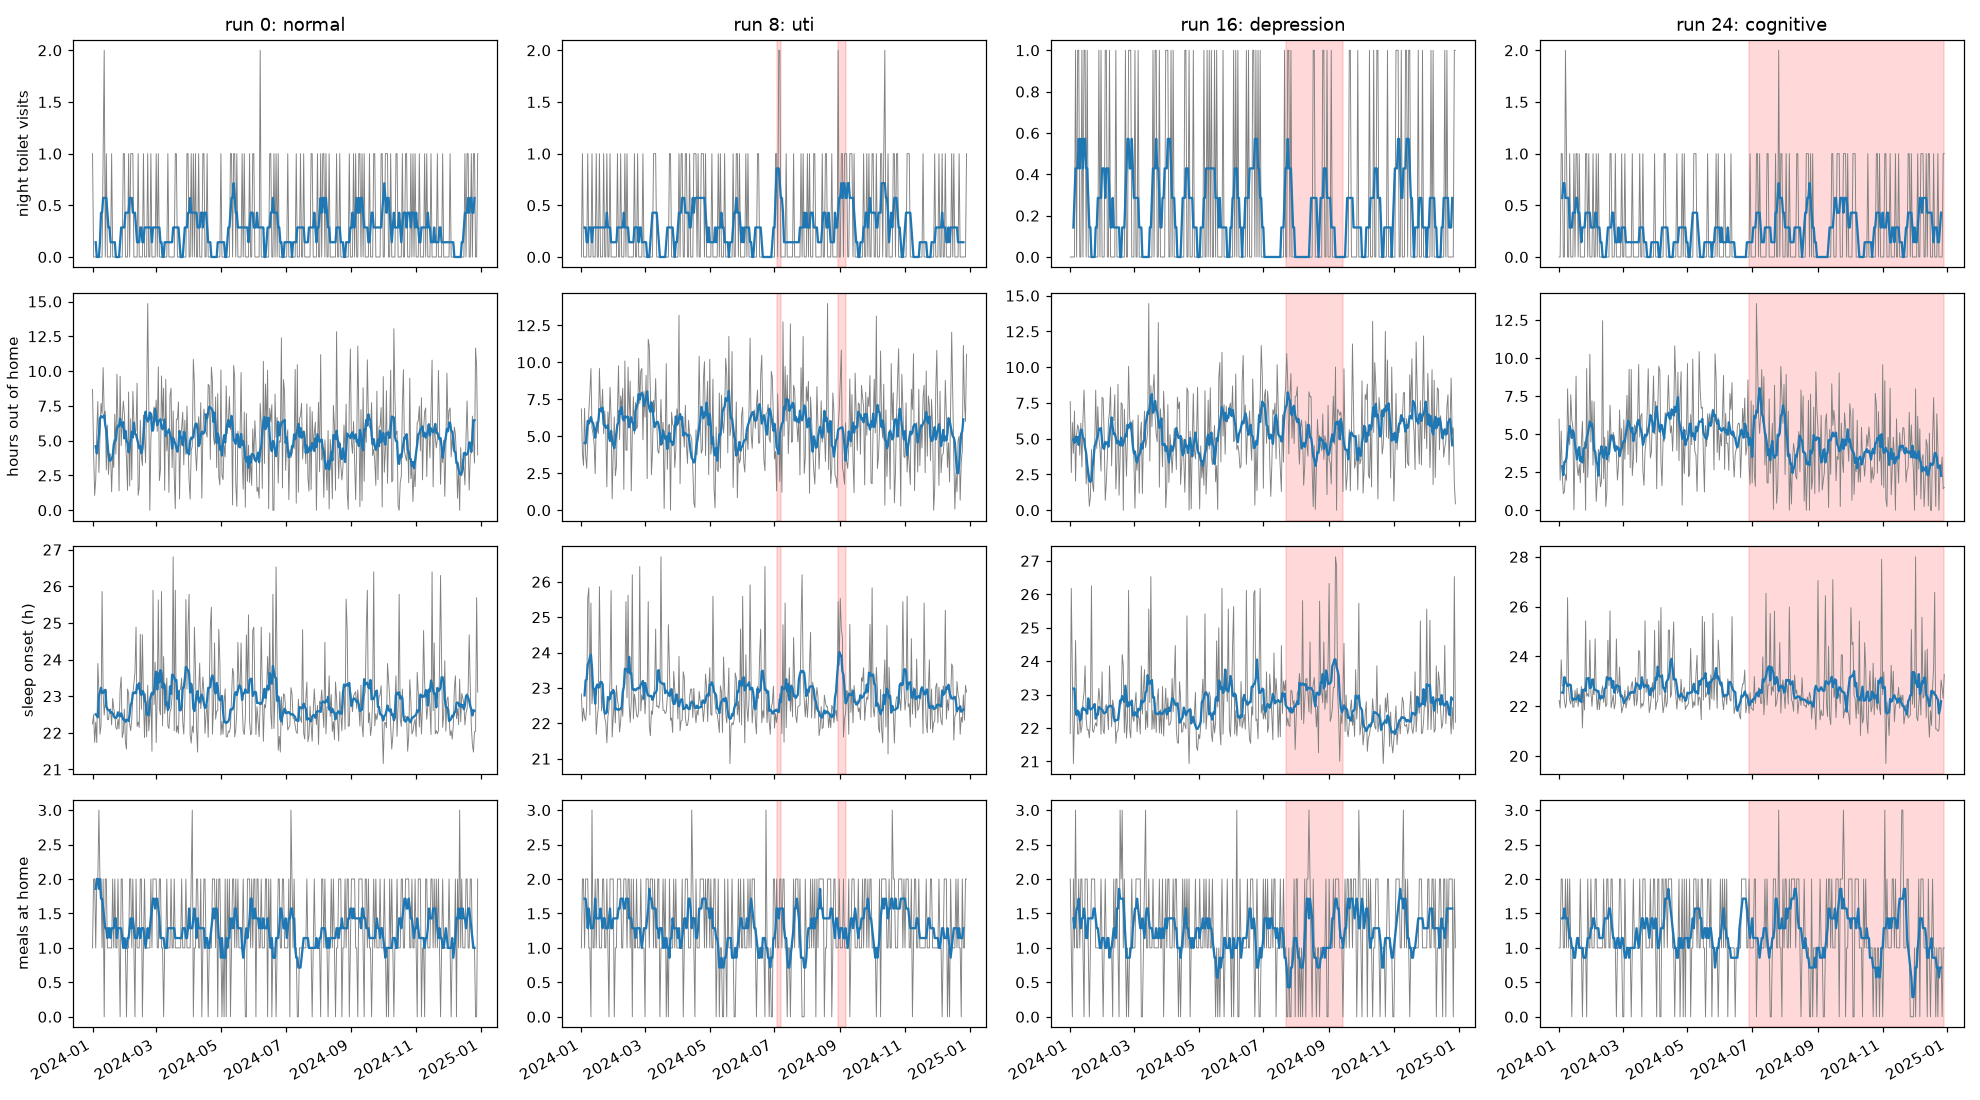
\includegraphics[width=0.49\linewidth]{t4_examples_hh113.png}\hfill
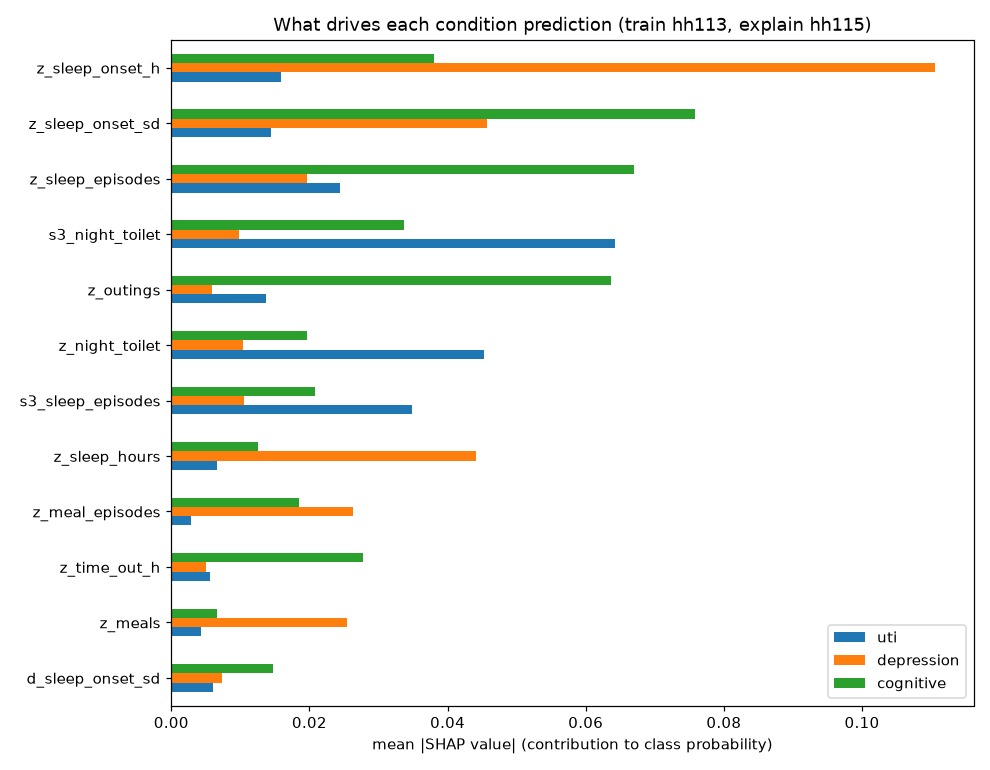
\includegraphics[width=0.40\linewidth]{t7_shap_importance.png}
\caption{Left: one simulated year per condition (red = injected episode). Right: mean $|$SHAP$|$ per condition (model trained on hh113, explained on hh115).}
\label{fig:shap}
\end{figure}

\subsection{Report level and real residents (O3)}
We simulated 32 new people (new seeds, never used in training) and produced a report every 35 days.
Table~\ref{tab:report} shows the trade-off at report level. A day-level calibration of 0.5 false alarms per 30 days made
about 55\% of normal 35-day reports show a change. After report-level calibration, most normal reports are clean, but
sensitivity per report is modest, especially for the gradual conditions. With the \emph{initial} reference, a slow
decline stays visible, but on the real residents habit drift makes hh113 ``cognitive'' in most reports. The
\emph{rolling} reference avoids this but absorbs slow decline. We therefore use \emph{rolling} by default and always show
the long-term trend against the initial habits.

\begin{figure}[h]
\centering
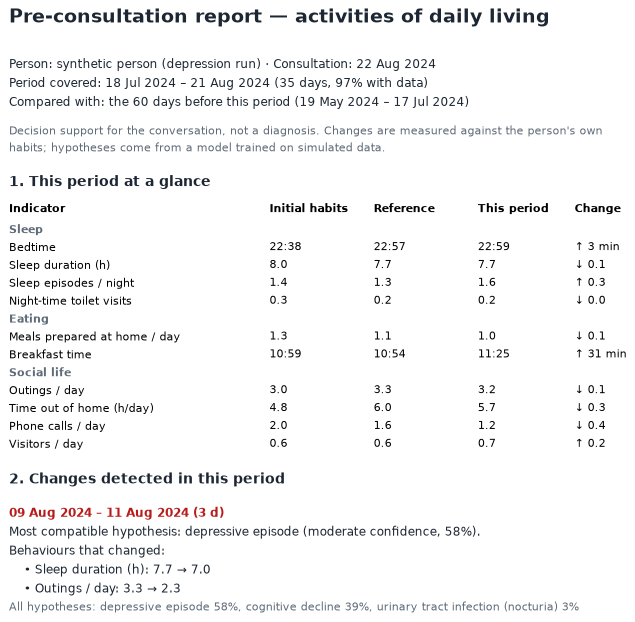
\includegraphics[width=0.62\linewidth]{report_example.png}
\caption{First page of a generated report (PDF) for a held-out synthetic person with a depressive episode (onset 22~Jul).
The long-term chart is on page 2. The supporting behaviours are those that moved at least $1\sigma$ in the expected direction.}
\label{fig:report}
\end{figure}

\begin{table}[h]
\centering\small
\begin{tabular}{llcccc}
\toprule
Reference & Truth (reports) & Sensitivity & Correct & Clean normal & Wrong claim \\
\midrule
rolling & cognitive (56) & 25\% & 16\% & -- & 2\% \\
rolling & depression (17) & 29\% & 6\% & -- & 12\% \\
rolling & normal (165) & -- & -- & 83\% & 8\% \\
rolling & uti (18) & 39\% & 28\% & -- & 17\% \\
\midrule
initial & cognitive (56) & 38\% & 36\% & -- & 2\% \\
initial & depression (17) & 35\% & 12\% & -- & 24\% \\
initial & normal (165) & -- & -- & 78\% & 13\% \\
initial & uti (18) & 67\% & 33\% & -- & 17\% \\
\midrule
initial & real hh113 (12) & \multicolumn{4}{l}{75\% of reports name a condition; 9 name cognitive decline} \\
rolling & real hh113 (12) & \multicolumn{4}{l}{25\% of reports name a condition; 2 name cognitive decline} \\
initial & real hh115 (7) & \multicolumn{4}{l}{14\% of reports name a condition; 1 name cognitive decline} \\
rolling & real hh115 (7) & \multicolumn{4}{l}{29\% of reports name a condition; 1 name cognitive decline} \\
\bottomrule
\end{tabular}

\caption{Report-level evaluation on 32 fresh synthetic people (35-day reports). Sensitivity: a change is reported when
the condition is active for at least 3 days of the period. Correct: the report names it. Wrong claim: the report names a
condition that is not active. Real residents: share of reports naming a condition.}
\label{tab:report}
\end{table}

% ---------------------------------------------------------------------------------------------------------------
\section{Discussion and limitations}
The pipeline follows the design of simulator-based detection for older adults living alone~\cite{tanaka2023simulation,tanaka2024detection},
with realism checked as in SynSys~\cite{dahmen2019synsys}, and adds evidence-tagged symptoms, a per-person baseline, a
cross-person test, clinician-oriented explanations and a sim-to-real check. The limitations are substantial and point to
future work.
\begin{itemize}\itemsep0pt
\item \textbf{Synthetic results are optimistic.} On real nurse-labelled events Isudra reaches G-mean 0.05--0.41~\cite{dahmen2021isudra}.
  We have no real labelled health events. The real-resident reports cannot be scored.
\item \textbf{Symptom magnitudes} are partly assumptions. Notably, the UTI effect size on night toilet visits has no
  quantitative source yet. Population coefficients~\cite{petersen2015timeout} are applied within one person.
\item \textbf{Simulator.} Two homes, one resident each; stationary habits (no drift, unlike real data); some outings are
  dropped; conditions never overlap; no physiological signals (e.g.\ respiratory rate, key for UTI~\cite{capstick2024uti}).
\item \textbf{Detection} thresholds transfer only roughly between persons. Personal calibration and calibrated
  uncertainty with abstention~\cite{ugwu2026clinician} are needed.
\item \textbf{Report} usefulness was not evaluated with clinicians. A survey such as~\cite{ugwu2026clinician} is the next step.
\end{itemize}

\section{Conclusion and next steps}
A small, transparent pipeline can turn an event list into a periodic pre-consultation report, and its components can
be checked one by one against prior work. The main lessons are quantitative: synthetic data can match real habits as
well as the same person's next year does; per-person attribution transfers to an unseen person; but at a false-report
rate a GP would accept, gradual conditions are hard to see within 35 days, and real habit drift must be handled
explicitly. For ObsAVQ, next steps are: events from audio recognition~\cite{vacher2011audio}, simulation with drift and
comorbidity, personal thresholds with calibrated uncertainty, evaluation with GPs, and optional LLM rephrasing of
verified facts only~\cite{fiori2025llm}.

\bibliographystyle{unsrtnat}
\bibliography{refs}
\end{document}
